% ============================================================
% tikz_tan6.tex —— 探六例1 正方体图（TikZ 矢量重绘，独立件）
% 源：工作区/字替对照-0909/variantF/media/media/image3.png（521×496px）
% 源排印：86.0×82.0mm（源文件 image3 明确宽高各定，横 86/521=0.165067mm/px，纵 82/496=0.165323mm/px）
% 题：在正方体 ABCD-A₁B₁C₁D₁ 中，求向量 BC₁ 与 AC 的夹角
%     （黑粗线 BC₁、AC、AD₁、D₁C = 所问向量及其平移辅助，构成等边△ACD₁）
% 编译：xelatex tikz_tan6.tex（或 pdflatex；仅依赖 tikz，standalone 类）
% ------------------------------------------------------------
% 坐标系：1 单位 = 1mm，原点 = 源图左下角；页 = 86×82mm（与源排印同尺）
% 几何（按源逐像素实测并校正线心，与实测偏差 ≤0.2mm）：
%   正面矩形 49.60(宽)×49.74(高)（源图纵横比 0.16% 拉伸＋顶前棱微倾所致）；
%   深度位移 ≈ (+17.50, +17.45)mm（≈45°，斜二测方向）
%   A(9.25,7.05)  B(58.85,7.05)  C(76.35,24.55)  D(26.75,24.55)
%   A1(9.25,56.79) B1(58.85,56.68) C1(76.35,74.17) D1(26.75,74.17)
% ------------------------------------------------------------
% 线宽折算（1px = 0.165mm）：
%   灰线（正方体棱，源墨色 #404040 = K25，= black!75）实测 2.62px → 0.43mm（≈1.22pt）
%   黑线（BC₁/AC/AD₁/D₁C 四段强调线）实测 3.55px → 0.59mm（≈1.66pt）
% 虚线折算：实段 11px、空段 8.5px → on 1.82mm / off 1.40mm（源黑白虚线同规，黑线略长系墨深阈值效应）
% 标签字号折算：大写高实测 25.5px → 4.21mm ⇒ 数学体 17.5pt（CM cap 0.683em ≈ 4.10mm，差 2.5%），下标自动
%   注：标签用裸数学体（项目先例：练习件样张 $A_1$ 直排）；集成进本件（unicode-math + TeX Gyre Termes Math）
%   即为 Times 系观感，与源图一致。
% ============================================================
\documentclass[tikz,border=0pt]{standalone}
\definecolor{cubegray}{gray}{0.25}   % 源灰墨 #404040
\begin{document}
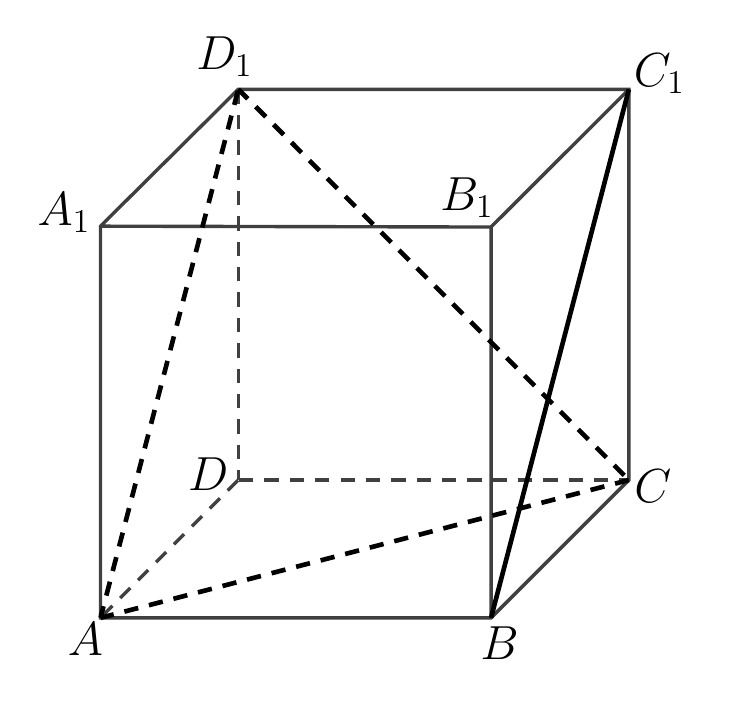
\begin{tikzpicture}[x=1mm,y=1mm,
    line width=0.43mm, line cap=butt, line join=miter,
    every node/.style={inner sep=0pt,outer sep=0pt},
    lab/.style={font=\fontsize{17.5}{21}\selectfont}]
  \useasboundingbox (0,0) rectangle (86,82);

  % ---- 顶点 ----
  \coordinate (A)  at ( 9.25, 7.05);
  \coordinate (B)  at (58.85, 7.05);
  \coordinate (C)  at (76.35,24.55);
  \coordinate (D)  at (26.75,24.55);
  \coordinate (A1) at ( 9.25,56.79);
  \coordinate (B1) at (58.85,56.68);
  \coordinate (C1) at (76.35,74.17);
  \coordinate (D1) at (26.75,74.17);

  % ---- 灰线·实线棱（9 段）----
  \draw[cubegray] (A)--(B)--(C)--(C1)--(D1)--(A1)--cycle % 底前棱、底右棱、右后棱、顶后棱、顶左棱、左前棱
                  (A1)--(B1)--(B)                        % 顶前棱、右前棱
                  (B1)--(C1);                            % 顶右棱
  % ---- 灰线·虚线棱（3 段隐藏棱：AD、DC、DD₁）----
  % dash phase = 按源图虚线节距逐段反解的对相（锚点=笔画起端；on 1.82 / off 1.40mm，周期 3.22mm）
  \draw[cubegray,dash pattern=on 1.82mm off 1.40mm,dash phase=2.90mm] (A)--(D);
  \draw[cubegray,dash pattern=on 1.82mm off 1.40mm,dash phase=0.62mm] (C)--(D);
  \draw[cubegray,dash pattern=on 1.82mm off 1.40mm,dash phase=3.18mm] (D1)--(D);

  % ---- 黑粗线（问题向量及其平移辅助：BC₁ 实线；AC、AD₁、D₁C 虚线）----
  \draw[line width=0.59mm] (B)--(C1);
  \draw[line width=0.59mm,dash pattern=on 1.82mm off 1.40mm,dash phase=0.09mm] (A)--(C);
  \draw[line width=0.59mm,dash pattern=on 1.82mm off 1.40mm,dash phase=0.30mm] (A)--(D1);
  \draw[line width=0.59mm,dash pattern=on 1.82mm off 1.40mm,dash phase=0.11mm] (D1)--(C);

  % ---- 顶点标签（位置 = 源图墨迹中心，mm）----
  \node[lab] at ( 4.62,58.48) {$A_1$};
  \node[lab] at ( 7.35, 4.38) {$A$};
  \node[lab] at (59.93, 3.80) {$B$};
  \node[lab] at (55.80,60.43) {$B_1$};
  \node[lab] at (80.22,76.13) {$C_1$};
  \node[lab] at (79.40,23.72) {$C$};
  \node[lab] at (22.94,25.29) {$D$};
  \node[lab] at (25.01,78.28) {$D_1$};
\end{tikzpicture}
\end{document}
